\documentclass[12pt]{article}
\usepackage{scrextend}
\usepackage[utf8]{inputenc}
\usepackage[polish]{babel}
\usepackage[T1]{fontenc}%polskie znaki
\usepackage[utf8]{inputenc}%polskie znaki
\usepackage{geometry}
\usepackage{float}
\usepackage{enumitem}
\usepackage{hyperref}
\usepackage{graphicx}
\usepackage{tabulary}
\usepackage{etoc}
\usepackage[normalem]{ulem} 
\renewcommand{\baselinestretch}{1.5}
\graphicspath{ {img/} }
\newgeometry{lmargin=2cm, rmargin=2cm, tmargin=2cm, bmargin=2cm}
\usepackage{tikz}
\usepackage[bf]{caption}
\usepackage{setspace}
\usepackage{rotating}
\newcommand{\scenario}[5]{
  \subsection{#1}
  \begin{minipage}{\textwidth}
    \textbf{Cel:} #2 \\
    \textbf{WS:} #3 \\
    \textbf{WK:} #4 \\
    \textbf{Przebieg:}
    \begin{enumerate}
      \setlength\itemsep{0.0em}
      #5
    \end{enumerate}
  \end{minipage}
}
\hyphenation{include}
\hyphenation{extend}



\usepackage{listings}
\usepackage{xcolor}
 
\definecolor{codegreen}{rgb}{0,0.6,0}
\definecolor{codegray}{rgb}{0.5,0.5,0.5}
\definecolor{codepurple}{rgb}{0.58,0,0.82}
\definecolor{backcolour}{rgb}{0.99,0.99,0.973}
 
\lstdefinestyle{mystyle}{
    backgroundcolor=\color{backcolour},   
    commentstyle=\color{codegreen},
    keywordstyle=\color{magenta},
    numberstyle=\tiny\color{codegray},
    stringstyle=\color{codepurple},
    basicstyle=\ttfamily\footnotesize,
    breakatwhitespace=false,         
    breaklines=true,                 
    captionpos=b,                    
    keepspaces=true,                 
    numbers=left,                    
    numbersep=5pt,                  
    showspaces=false,                
    showstringspaces=false,
    showtabs=false,                  
    tabsize=2
}
\lstset{
    extendedchars=false,
    inputencoding=utf8
}
\renewcommand{\lstlistlistingname}{Spis listingów}\lstset{style=mystyle}


\begin{document}

\begin{flushleft}
        Damian Koper, \textbf{241292} \\
        Łukasz Handschuh, \textbf{241402}
\end{flushleft}
\vspace{1cm}
{
    \centering
    {\Huge\scshape\bfseries Inżynieria oprogramowania - Etap 4 }\\
    \vspace{0.25cm}
    \Large\textbf{Dział ewidencji ludności} \\
    \vspace{0.25cm}
    \large Identyfikacja klas reprezentujących logikę biznesową
    projektowanego oprogramowania, definicja atrybutów i
    operacji klas oraz związków między klasami - na podstawie
    analizy scenariuszy przypadków użycia. Opracowanie
    diagramów klas i pakietów. Zastosowanie projektowych
    wzorców strukturalnych i wytwórczych.\\
}

\section{Przypadki użycia - zakres analizy}
W modelowaniu klas zastosowano wzorzec Model-View-Controller z separacją serwisów oraz wzorzec repozytorium. Analiza przeprowadzona została dla następujących przypadków użycia:
\begin{itemize}[noitemsep]
    \item Wyświetlanie wniosków,
    \item Zmiana kryterium wyświetlania wniosków,
    \item Edycja danych wniosku,
    \item Zmiana statusu wniosku, 
\end{itemize}

\section{Analiza wspólności}
\subsection{Encje}
Analiza wykryła jedną abstrakcyjną klasę encji bazowej \lstinline{RegistrationBase} - Dane meldunkowe. Zawiera ona dwa obiekty:
\begin{itemize}[noitemsep]
    \item \lstinline{RegistryPersonalData} - dane osobowe, liczebność 1:1
    \item \lstinline{RegistryAddressData} - dane adresowe, liczebność 1:1
\end{itemize}

\subsection{Główny przepływ sterowania}
Realizacja wszystkich przypadków użycia oparta jest o interfejs konsoli. 
Wykryto następujące klasy obsługujące przepływ sterowania w aplikacji:
\begin{itemize}[noitemsep]
    \item \lstinline{ConsoleEngine} - klasa przechowuje instancje wszystkich kontrolerów i jest z nimi powiązana relacją kompozycji,
    \item \lstinline{RegistryApplicationController}
\end{itemize}
Wszystkie klasy kontrolerów realizują interfejs \lstinline{IController}.

\subsection{Widoki}
Wykryto następujące klasy widoków używane do wyświetlania i odpytywania użytkownika o dane:
\begin{itemize}[noitemsep]
    \item \lstinline{RegistryApplicationIndexView} - Wyświetlanie i filtrowanie wszystkich wniosków,
    \item \lstinline{RegistryApplicationShowView} - Wyświetlanie pojedynczego wniosku,
    \item \lstinline
    {RegistryApplicationUpdateView} - Edytowanie pojedyncego wniosku.
\end{itemize}
\subsubsection{Data transfer objects}

\begin{itemize}[noitemsep]
    \item \lstinline{TableDTO} - wyświetlanie tabel,
    \item \lstinline{RegisterApplicationDTO} - dane wniosku,
    \item \lstinline{FilterDataDTO} - dane filtracji wniosków.
\end{itemize}

\subsection{PESEL}
Komunikację z systemem PESEL odpowiedzialenego za weryfikacje danych osobowych będzie realizować będzie klasa \lstinline{PecelFacade} realizująca interfejs \lstinline{IPeselFacade}.

\newpage

\section{Analiza zmienności}
\subsection{Encje}
Wykryto dwa podzbiory danych meldunkowych - wniosek i meldunek faktyczny.
Zidentyfikowano następujące klasy pochodne klasy \lstinline{RegistryApplicationBase}: 
\begin{itemize}[noitemsep]
    \item \lstinline{RegistryApplication} - Wniosek meldunkowy,
    \item \lstinline{Registration} - Meldunek.
\end{itemize}

\subsection{Przechowywanie danych}
Dla każdej encji wykryto klasę repozytorium, która zapewnia odpowiedni poziom abstrakcji przy pobieraniu i zapisywaniu danych:
\begin{itemize}[noitemsep]
    \item \lstinline{RegistryApplicationRepository}
    \item \lstinline{RegistrationRepository}
\end{itemize}
Wszystkie klasy repozytoriów realizują interfejs \lstinline{IRepository} i są powiązane z obiektami, które przechowują, relacją kompozycji.

\subsection{Logika biznesowa}
Dla każdej encji wykryto klasę serwisu, który realizuje operacje opisane w logice biznesowej przypadków użycia:
\begin{itemize}[noitemsep]
    \item \lstinline{RegistryApplicationService}
    \item \lstinline{RegistrationService}
\end{itemize}


\section{Wzorce projektowe}
\subsection{Flyweight}
Rolę obiektów Flyweight pełnią klasy \lstinline{RegistryAddressData} oraz \lstinline{RegistryPersonalData}. Abstrakcyjnym klientem tych klas jest klasa \lstinline{RegistrationBase}, z której dziedziczą klasy \lstinline{RegistryApplication} oraz \lstinline{Registration}.
\subsection{Singleton}
Serwisy są obiektami typu singleton posiadające tylko jedną instancję. Dostęp i zarządzanie nimi jest możliwy przez fasadę, którą implementuje klasa \lstinline{App}.
Zastosowanie tego wzorca ułatwi późniejsze testowanie i mockowanie implementacji serwisów. 
\subsection{Fasada}
Wzorzec fasada użyty został przy zdefiniowaniu klasy \lstinline{PeselFasade}, która udostępnia metody umożliwiające komunikację z zewnętrznym systemem. Późniejsza możliwość podmiany implementacji dzięki interfejsowi \lstinline{IPeselFacade} zapewnia możliwość komunikacji z zewnętrznym systemem w dowolny sposób.


\begin{sidewaysfigure}[h]
    \centering
    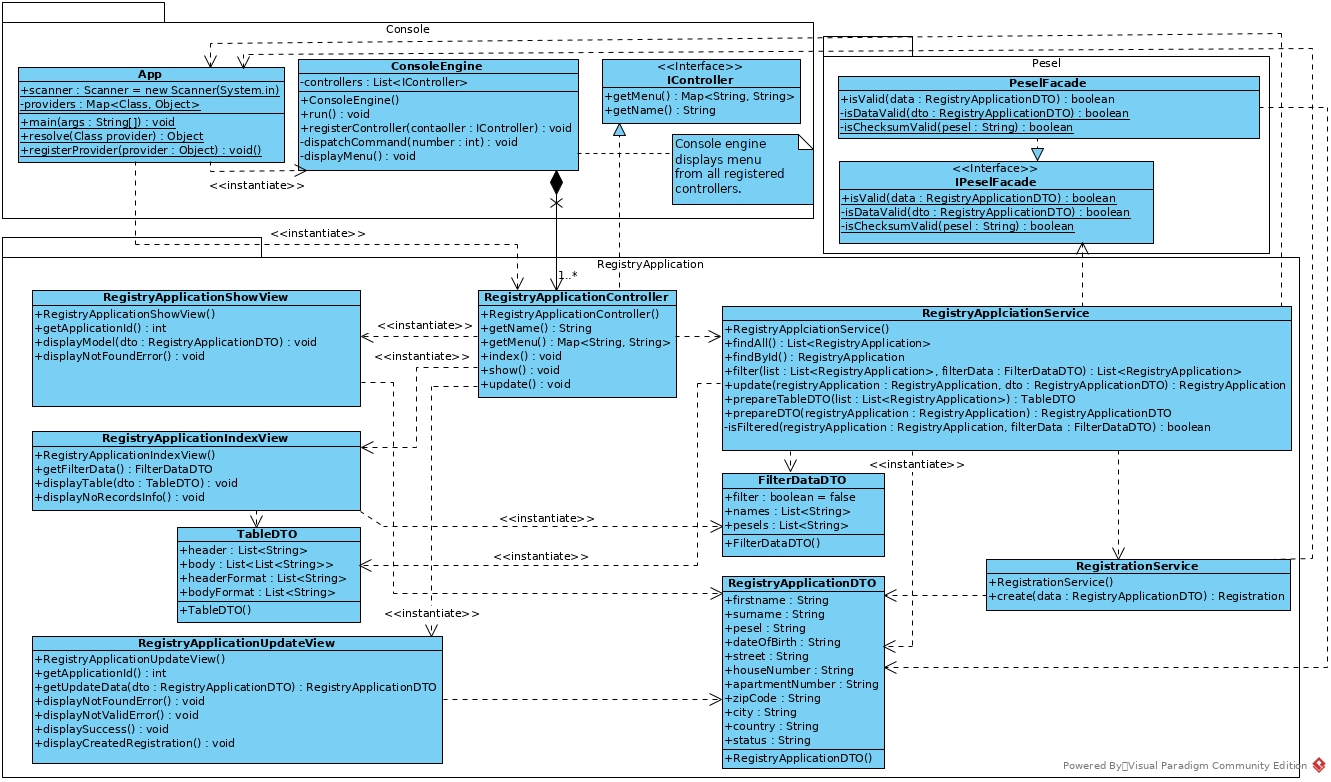
\includegraphics[
        keepaspectratio,
        width=\linewidth,
        height=\dimexpr\textheight-9\baselineskip
    ]{./../paragidm/export/PopulationRegistry_CD.jpg}
    \caption{Diagram klas - widoki, kontrolery i serwisy.}
    \label{}
\end{sidewaysfigure}

\begin{sidewaysfigure}[H]
    \centering
    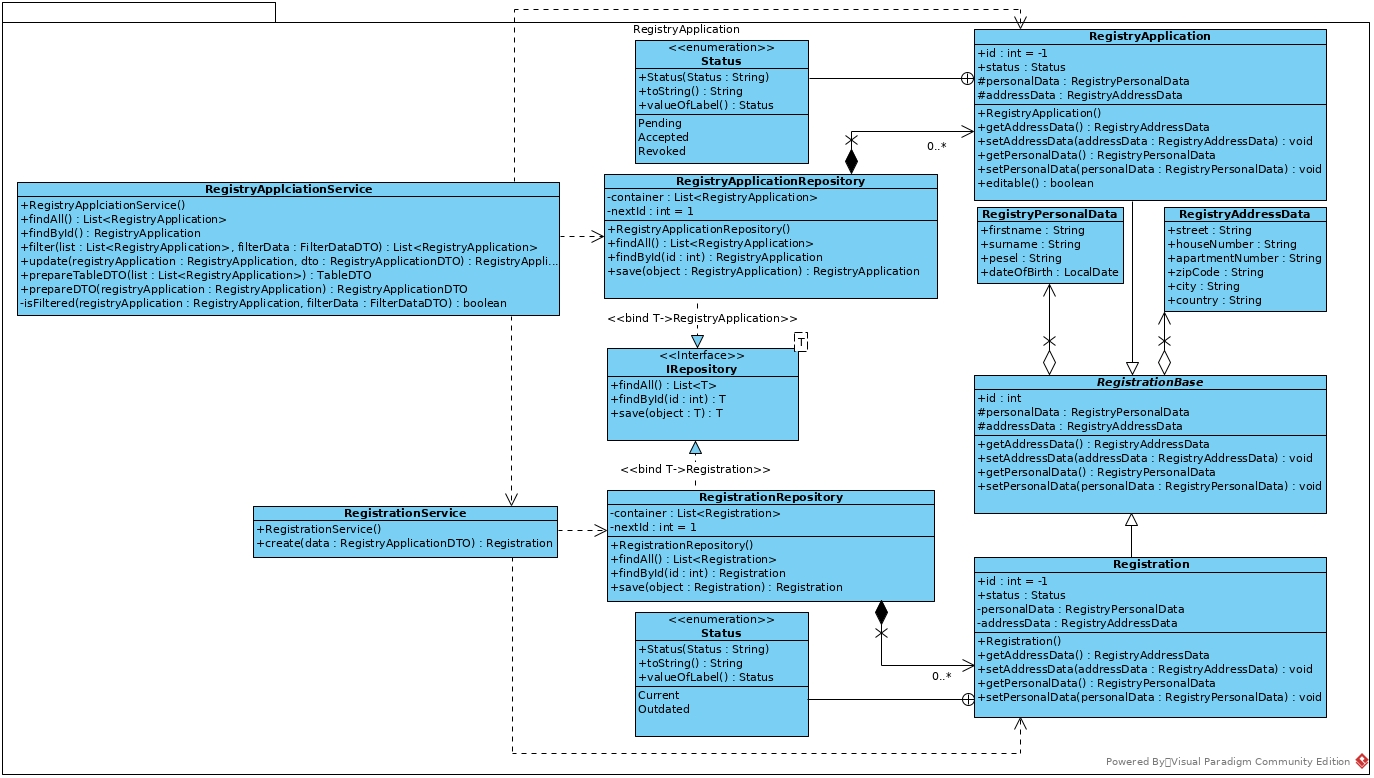
\includegraphics[
        keepaspectratio,
        width=\linewidth,
        height=\dimexpr\textheight-9\baselineskip
    ]{./../paragidm/export/PopulationRegistry_CD_1.jpg}
    \caption{Diagram klas - serwisy, repozytoria i encje.}
    \label{}
\end{sidewaysfigure}
\clearpage

\section{Diagramy sekwencji}
\subsection{Główna pętla sterowania}
\begin{figure}[H]
    \centering
    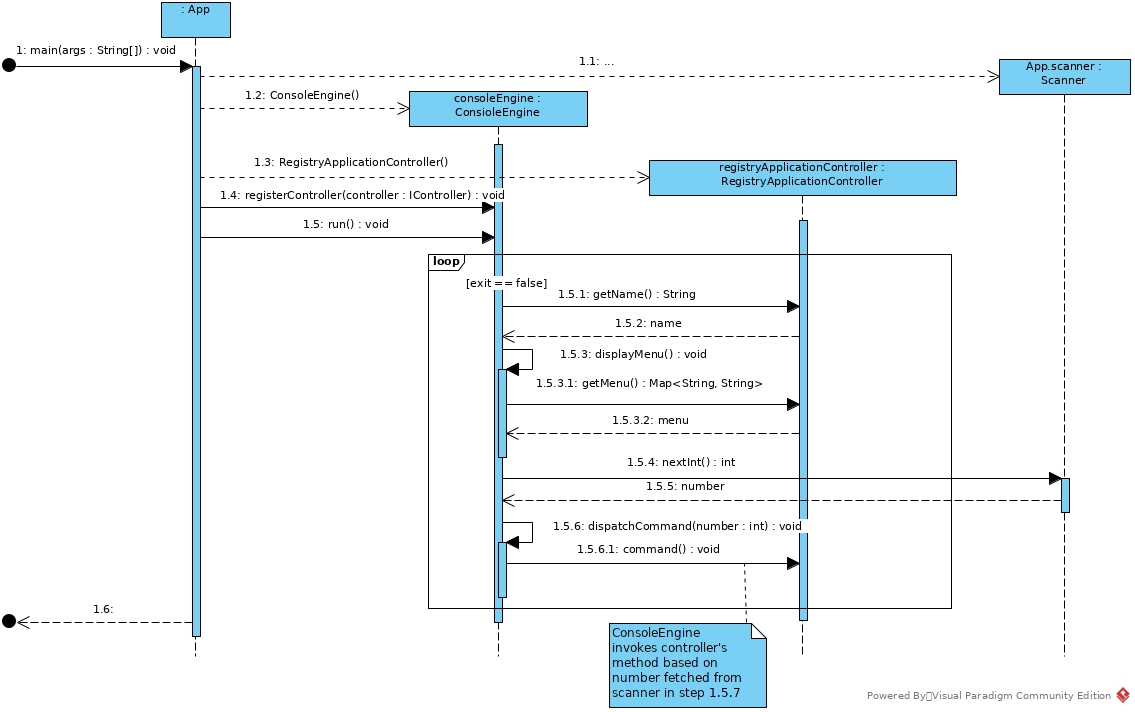
\includegraphics[
        keepaspectratio,
        width=\linewidth,
        height=\dimexpr\textheight-9\baselineskip
    ]{./../paragidm/export/Population_Regestry_SD_1.jpg}
    \caption{Diagram sekwencji - główna pętla przepływu sterowania.}
    \label{}
\end{figure}

\lstinputlisting[language=Java, firstline=20,lastline=47, caption=Metoda main klasy App]{../../src/main/java/populationRegistry/App.java}
\subsection{Wyświetlanie wniosków}
\begin{figure}[H]
    \centering
    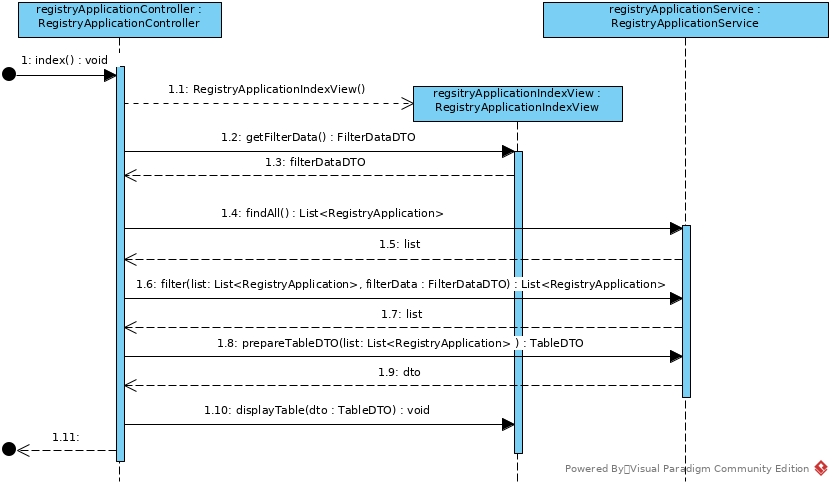
\includegraphics[
        keepaspectratio,
        width=\linewidth,
        height=\dimexpr\textheight-9\baselineskip
    ]{./../paragidm/export/Population_Registry_SD_2.jpg}
    \caption{Diagram sekwencji - wyświetlanie wniosków.}
    \label{}
\end{figure}

\lstinputlisting[language=Java, firstline=39,lastline=47, caption=Metoda index klasy RegistryApplicationController]{../../src/main/java/populationRegistry/registryApplication/controllers/RegistryApplicationController.java}

\subsection{Wyświetlanie pojedynczego wniosku}
\begin{figure}[H]
    \centering
    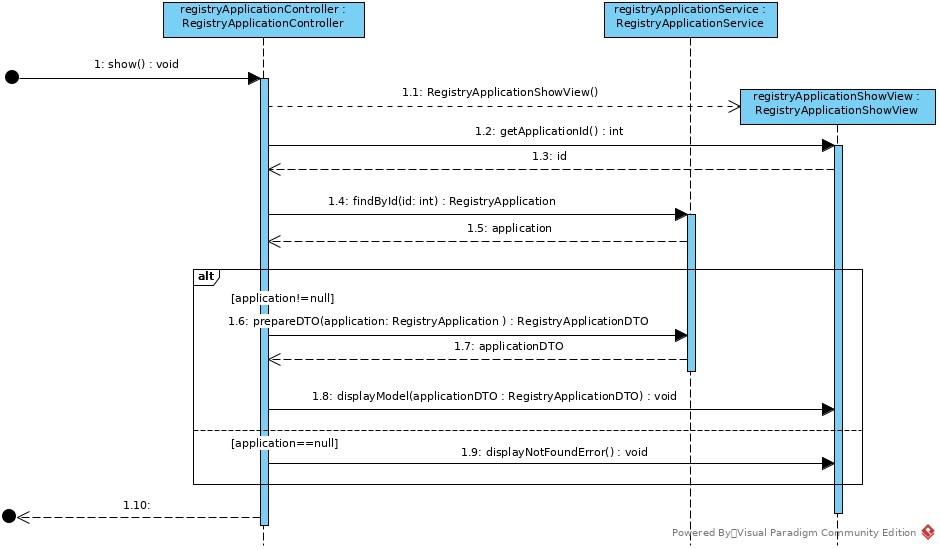
\includegraphics[
        keepaspectratio,
        width=\linewidth,
        height=\dimexpr\textheight-9\baselineskip
    ]{./../paragidm/export/Population_Registry_SD_3.jpg}
    \caption{Diagram sekwencji - wyświetlanie pojedynczego wniosku.}
    \label{}
\end{figure}

\lstinputlisting[language=Java, firstline=49,lastline=61, caption=Metoda show klasy RegistryApplicationController]{../../src/main/java/populationRegistry/registryApplication/controllers/RegistryApplicationController.java}

\subsection{Edycja danych wniosku}
\begin{figure}[H]
    \centering
    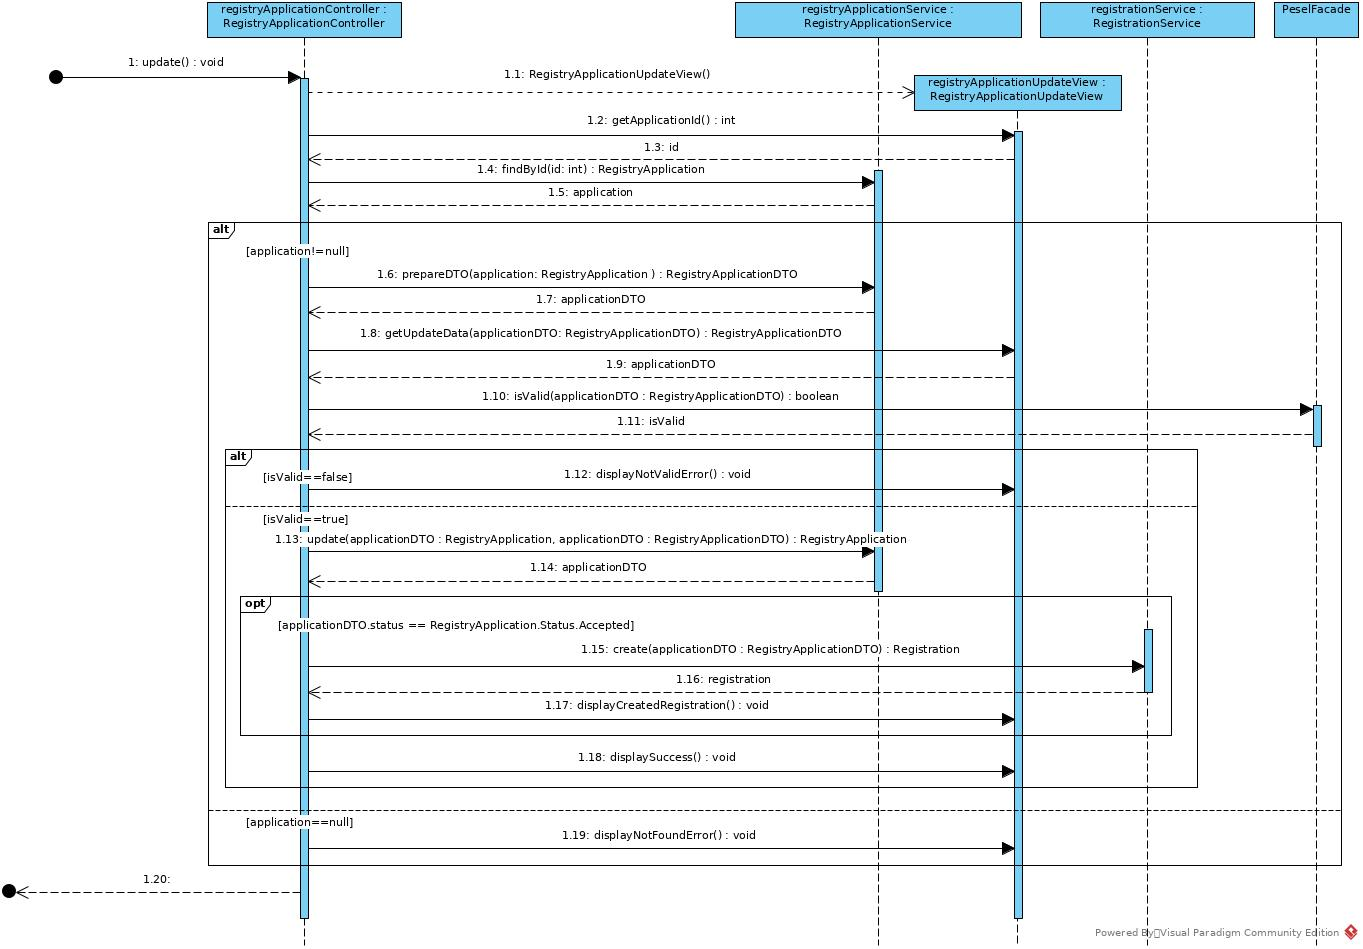
\includegraphics[
        keepaspectratio,
        width=\linewidth,
        height=\dimexpr\textheight-9\baselineskip
    ]{./../paragidm/export/Population_Registry_SD_4.jpg}
    \caption{Diagram sekwencji - edycja danych wniosku.}
    \label{}
\end{figure}

\lstinputlisting[language=Java, firstline=63,lastline=87, caption=Metoda update klasy RegistryApplicationController]{../../src/main/java/populationRegistry/registryApplication/controllers/RegistryApplicationController.java}


\subsection{Metody klasy RegistryApplicationService}
\begin{figure}[H]
    \centering
    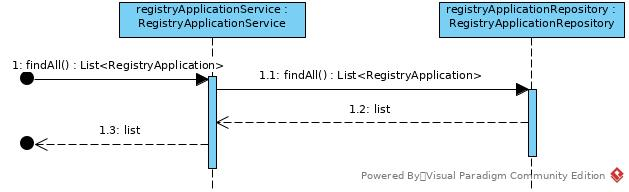
\includegraphics[
        keepaspectratio,
        width=\linewidth,
        height=\dimexpr\textheight-9\baselineskip
    ]{./../paragidm/export/Population_Registry_SD_5.jpg}
    \caption{Diagram sekwencji - metoda findAll klasy RegistryApplicationService.}
    \label{}
\end{figure}
\lstinputlisting[language=Java, firstline=22,lastline=26, caption=Metoda findAll klasy RegistryApplicationService]{../../src/main/java/populationRegistry/registryApplication/services/RegistryApplicationService.java}

\begin{figure}[H]
    \centering
    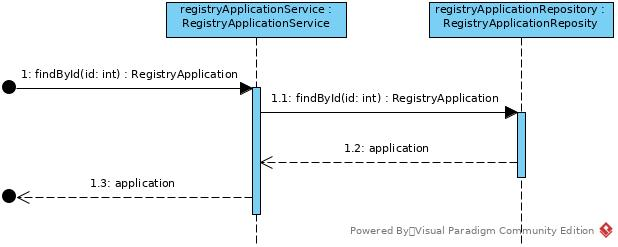
\includegraphics[
        keepaspectratio,
        width=\linewidth,
        height=\dimexpr\textheight-9\baselineskip
    ]{./../paragidm/export/Population_Registry_SD_6.jpg}
    \caption{Diagram sekwencji - metoda findById klasy RegistryApplicationService.}
    \label{}
\end{figure}
\lstinputlisting[language=Java, firstline=28,lastline=32, caption=Metoda findById klasy RegistryApplicationService]{../../src/main/java/populationRegistry/registryApplication/services/RegistryApplicationService.java}

\begin{figure}[H]
    \centering
    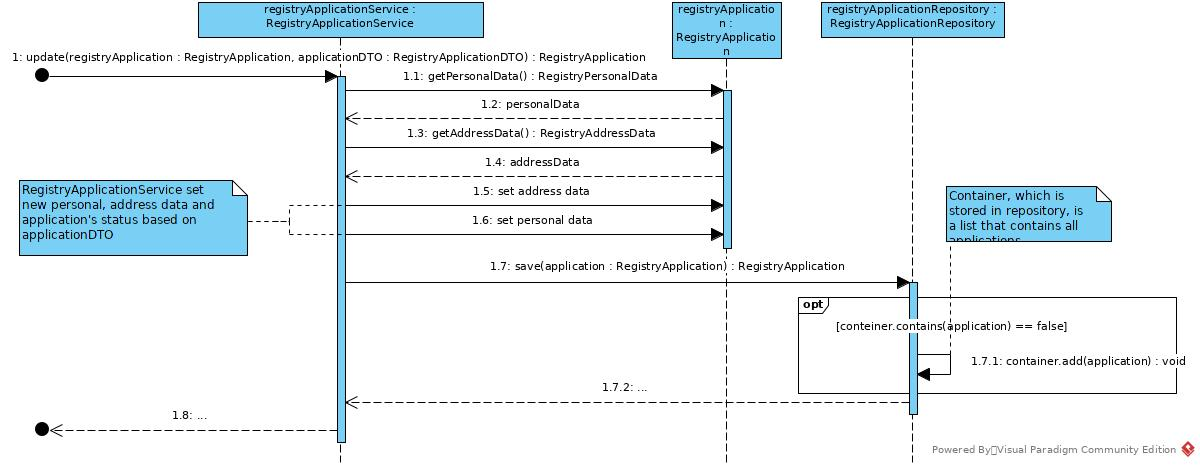
\includegraphics[
        keepaspectratio,
        width=\linewidth,
        height=\dimexpr\textheight-9\baselineskip
    ]{./../paragidm/export/Population_Registry_SD_7.jpg}
    \caption{Diagram sekwencji - metoda update klasy RegistryApplicationService.}
    \label{}
\end{figure}
\lstinputlisting[language=Java, firstline=64,lastline=84, caption=Metoda update klasy RegistryApplicationService]{../../src/main/java/populationRegistry/registryApplication/services/RegistryApplicationService.java}
\subsection{Metody klasy RegistrationService}
tutaj uzupełnić

\section{Kod źródłowy aplikacji}
\lstinputlisting[language=Java, caption=Klasa App]{../../src/main/java/populationRegistry/App.java}
\lstinputlisting[language=Java, caption=Interface IController]{../../src/main/java/populationRegistry/console/IController.java}
\lstinputlisting[language=Java, caption=Klasa ConsoleEngine]{../../src/main/java/populationRegistry/console/ConsoleEngine.java}
\lstinputlisting[language=Java, caption=Interface IPeselFacade]{../../src/main/java/populationRegistry/registryApplication/services/IPeselFacade.java}
\lstinputlisting[language=Java, caption=Klasa PeselFacade]{../../src/main/java/populationRegistry/pesel/PeselFacade.java}
\lstinputlisting[language=Java, caption=Interface IRepository]{../../src/main/java/populationRegistry/registryApplication/repositories/IRepository.java}
\lstinputlisting[language=Java, caption=Klasa RegistrationRepository]{../../src/main/java/populationRegistry/registryApplication/repositories/RegistrationRepository.java}
\lstinputlisting[language=Java, caption=Klasa RegistryApplicationRepository]{../../src/main/java/populationRegistry/registryApplication/repositories/RegistryApplicationRepository.java}
\end{document}
